\section{Simulation Results and Analysis} \label{sec:SimulationResultsAnalysis}

This section presents the analysis of the simulation results. A simulated scenario is considered successful if the resulting implied volatility surface satisfies all five quality criteria. These criteria are motivated by empirical stylized facts observed in financial markets and are designed to assess whether a simulated surface can be regarded as realistic.

First, the quality criteria are formally defined. Next, a ceteris paribus analysis is conducted to isolate the effect of individual model parameters. Finally, the simulation output is evaluated across a broad set of parameter constellations, and parameter ranges with high success rates are identified.


\subsection{Simulation Quality Criteria} \label{subsec:SimulationQualityCriteria}

Based on empirical observations in financial markets, five quality criteria are defined to assess the plausibility of simulated implied volatility surfaces:
\begin{itemize}
    \item Put-call parity must hold.
    \item The implied volatility smile must exhibit convexity.
    \item The at-the-money (ATM) volatility skew should be negative.
    \item The ATM skew should increase with time to maturity.
    \item The ATM skew term structure should decay approximately according to a power law.
\end{itemize}
A simulation scenario is considered successful if the corresponding implied volatility surface satisfies all five quality criteria.

\subsubsection*{Put-Call Parity Criterion}
The put-call parity (see \citealp{Björk2009}) establishes a fundamental no-arbitrage relationship between the prices of European call and put options. At time $t$, it states:
\begin{equation} \label{eq:PutCallParity}
    C_t - P_t = S_t - K \cdot B(t,T),
\end{equation}
where $C_t$ and $P_t$ denote the prices of a European call and put option with strike $K$ and maturity $T \geq t$, $S_t$ is the spot price of the underlying asset, and $B(t,T) = e^{-r(T - t)}$ is the discount factor under a constant risk-free rate $r$.

In the simulation, this relation is evaluated at $t = 0$. The element-wise relative deviation from parity is computed as:
\begin{equation} \label{eq:PutCallViolation}
    \text{Relative Error}_{l,q} = \left| \frac{C_0^{(l,q)} - P_0^{(l,q)} - \left( S_0 - K_l e^{-r T_q} \right)}{S_0} \right|,
\end{equation}
where the indices $(l, q)$ refer to the strike $K_l$ and maturity $T_q$.

A simulation scenario satisfies the put-call parity criterion if the mean relative deviation across all $(l, q)$ does not exceed 0.1\% and the maximum violation does not exceed 0.5\%. Satisfying this condition ensures internal consistency between simulated call and put prices, justifying their aggregation into a single implied volatility surface.

\subsubsection*{Smile Convexity Criterion}
In financial markets, implied volatility typically exhibits a smile-shaped pattern across strikes for a fixed maturity: volatility tends to be lowest at-the-money and higher for deep in- or out-of-the-money options. To assess this convexity, a quadratic polynomial is fitted to the implied volatilities for each maturity.

If the fitted parabola has a positive leading coefficient and an $R^2$-value above 90\%, the smile is considered convex at that maturity. The criterion is satisfied if this convex smile pattern is observed for the shortest maturity and for at least 90\% of all maturities overall.


\subsubsection*{ATM Skew Negativity Criterion}
Empirically, the ATM volatility skew tends to be negative, meaning that implied volatility decreases with increasing moneyness around the at-the-money level. The ATM skew is defined as in \citet{BayerFrizGatheral2016} by
\begin{equation} \label{eq:ATMSkew}
    \psi(\tau) := \left. \frac{\partial}{\partial k} \sigma_{\text{BS}}(k, \tau) \right|_{k = 0},
\end{equation}
where $\sigma_{\text{BS}}(k, \tau)$ is the implied Black-Scholes volatility for log-moneyness $k$ and maturity $\tau$.

The ATM skew negativity criterion is satisfied if $\psi(\tau) < 0$ for at least 90\% of the maturities.

\subsubsection*{ATM Skew Increase Criterion}
It is commonly observed that the magnitude of the ATM skew diminishes with increasing maturity, resulting in a flatter term structure. Hence, the ATM skew function $\psi(\tau)$ is expected to increase with maturity, i.e., become less steep for longer maturities.

This behavior is tested by fitting a linear regression to $\psi(\tau)$ across maturities. If the slope of the fitted line is positive, the criterion is considered satisfied.

\subsubsection*{ATM Skew Power Law Criterion}
Empirical studies suggest that the ATM skew decays approximately as a power law (see \citealp{Fukasawa2011} and \citealp{GatheralJaissonRosenbaum2018}) of the form:
\begin{equation} \label{eq:PowerLaw}
    \psi(\tau) \sim \tau^{-\gamma},
\end{equation}
with $\gamma = \tfrac{1}{2} - H$. To test for this behavior, a linear regression is performed on the log-log plot of $\psi(\tau)$ versus $\tau$. This corresponds to testing whether $\log \psi(\tau)$ is approximately linear in $\log(\tau)$.

The power law criterion is satisfied if the resulting regression model achieves an $R^2$-value greater than 90\%.


\subsection{Individual Parameter Effects} \label{subsec:IndividualParameterEffects}

This section analyzes how changing one model parameter, while keeping all others fixed, affects the shape of the implied volatility surface and the values of the simulation quality criteria. The analysis is conducted in a ceteris paribus fashion and provides intuition for the results of the full parameter sweep in later sections.

\subsubsection*{Effect of the Roughness Parameter $H$}
For lower values of $H$ (i.e., rougher sample paths), the short-term ATM skew tends to decrease in magnitude. Additionally, the slope of the log-log regression fitted to the ATM skew term structure flattens, indicating that the power-law exponent decreases in absolute value as $H$ decreases.
\begin{figure}[H]
    \centering
    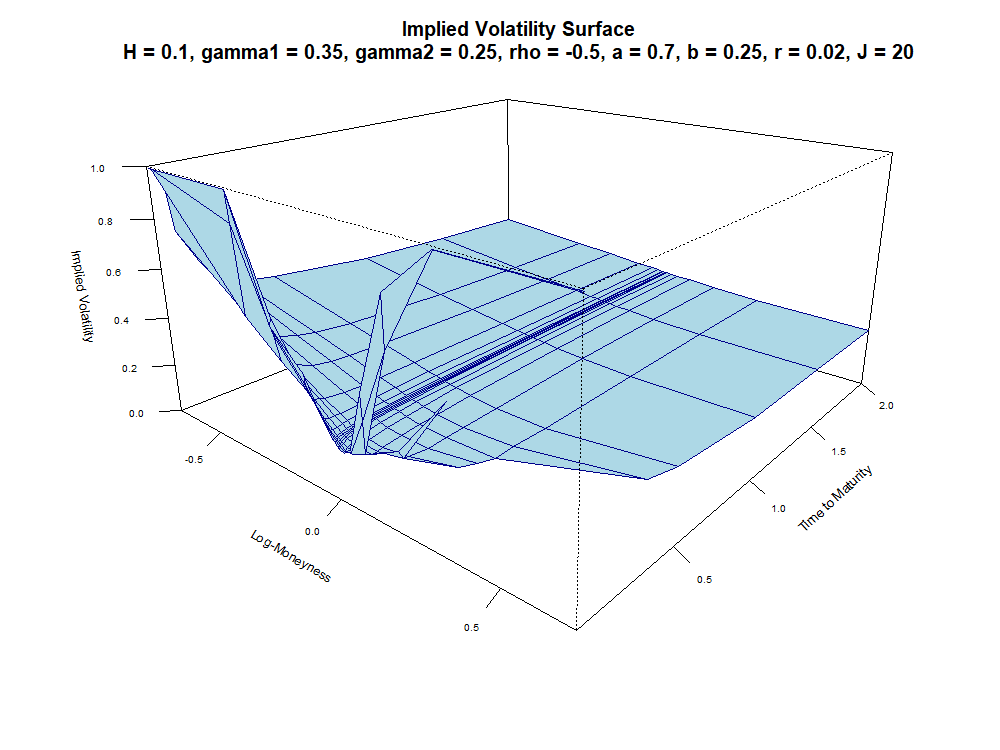
\includegraphics[width=0.45\textwidth]{figures/5.2 Individual Parameter Effects/H=0.10_iv_surface.png}
	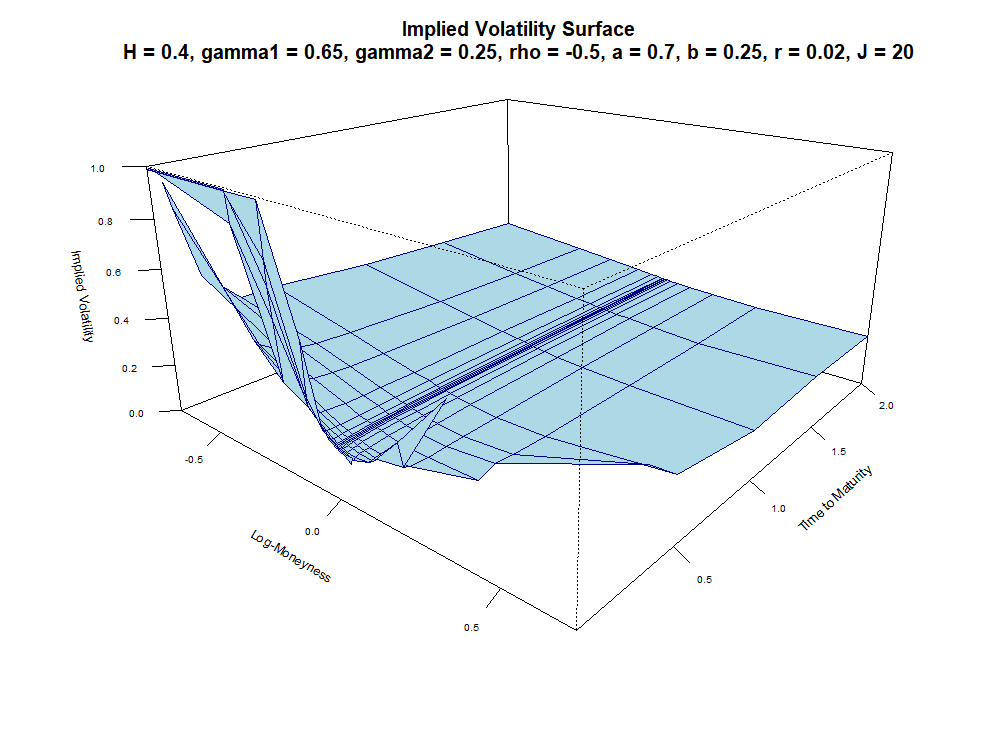
\includegraphics[width=0.45\textwidth]{figures/5.2 Individual Parameter Effects/H=0.40_iv_surface.png}
	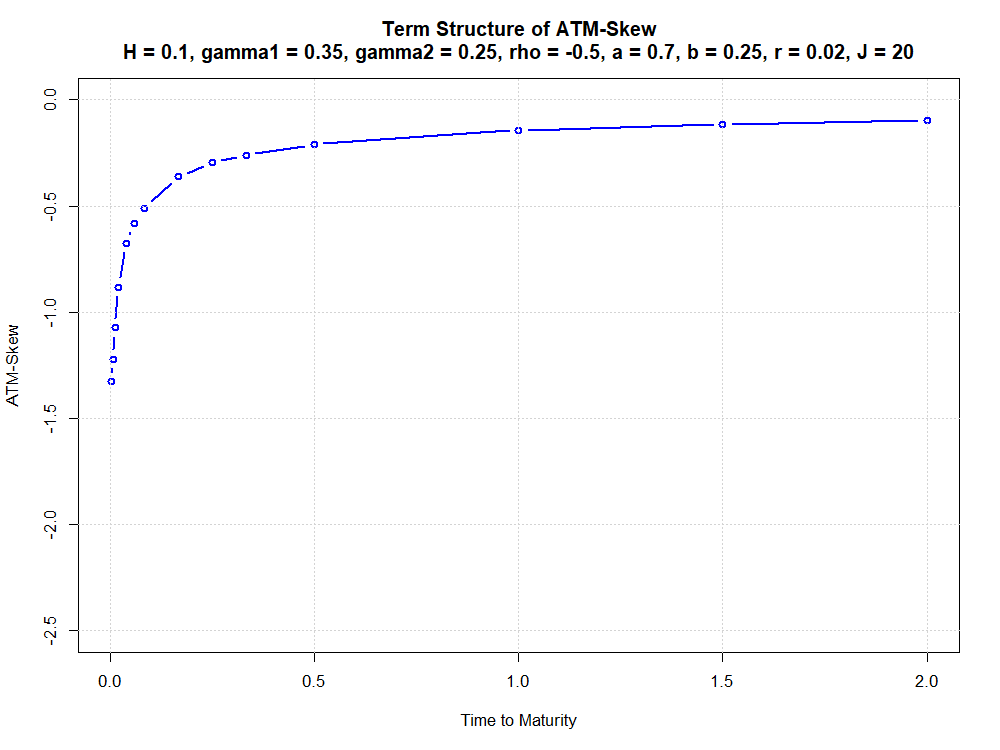
\includegraphics[width=0.45\textwidth]{figures/5.2 Individual Parameter Effects/H=0.10_atm_skew.png}
	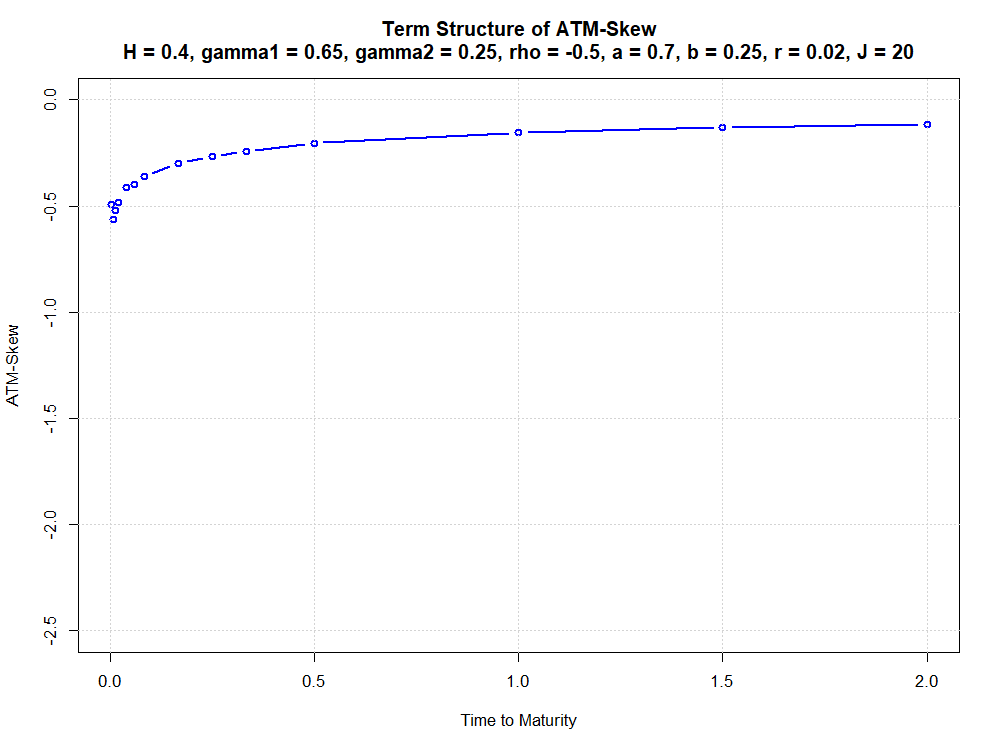
\includegraphics[width=0.45\textwidth]{figures/5.2 Individual Parameter Effects/H=0.40_atm_skew.png}
    \caption{Effect of roughness index $H$ on the implied volatility surface. Left: $H=0.10$. Right: $H=0.40$.}
    \label{fig:H_effect}
\end{figure}

\subsubsection*{Effect of Correlation Parameter $\rho$}
Decreasing the correlation $\rho$ between the Brownian motions driving the asset price and the volatility process (i.e., increasing the leverage effect) introduces a rightward tilt in the implied volatility surface. This results in lower implied volatilities for positive log-moneyness and higher volatilities for negative log-moneyness. As a consequence, the ATM skew increases in magnitude.
\begin{figure}[H]
    \centering
    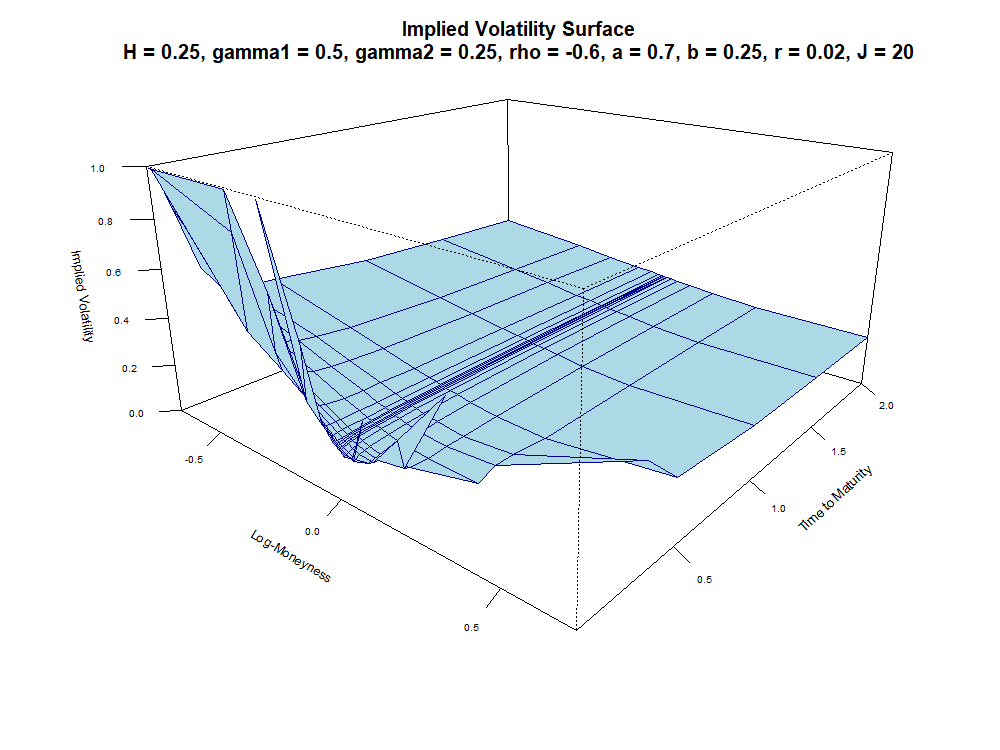
\includegraphics[width=0.45\textwidth]{figures/5.2 Individual Parameter Effects/rho=-0.6_iv_surface.png}
	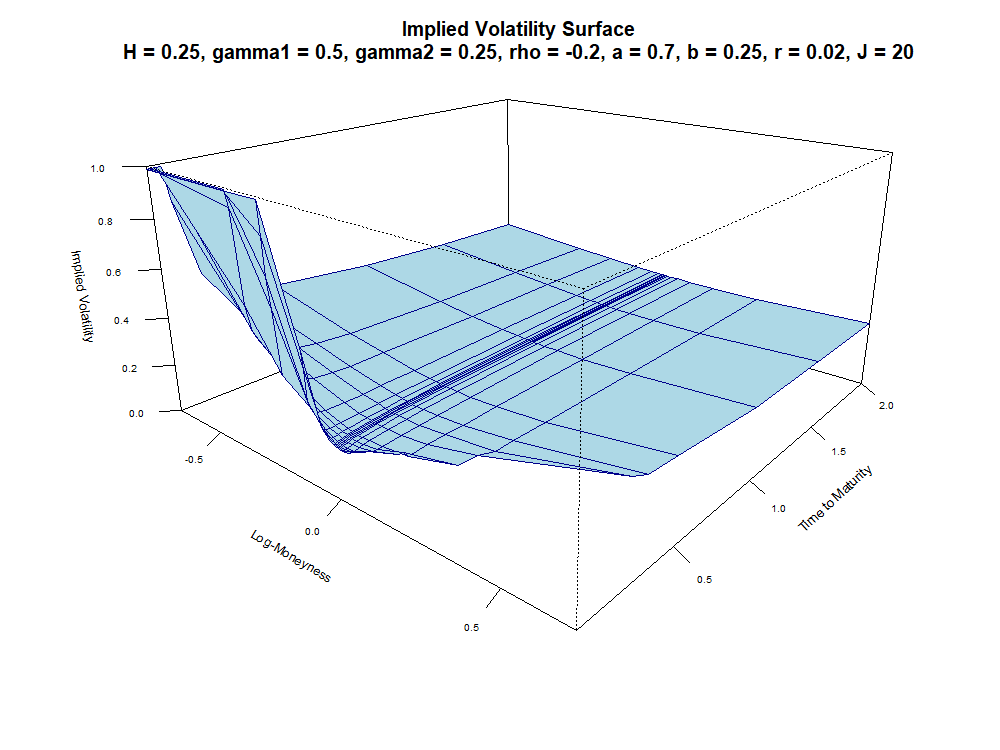
\includegraphics[width=0.45\textwidth]{figures/5.2 Individual Parameter Effects/rho=-0.2_iv_surface.png}
	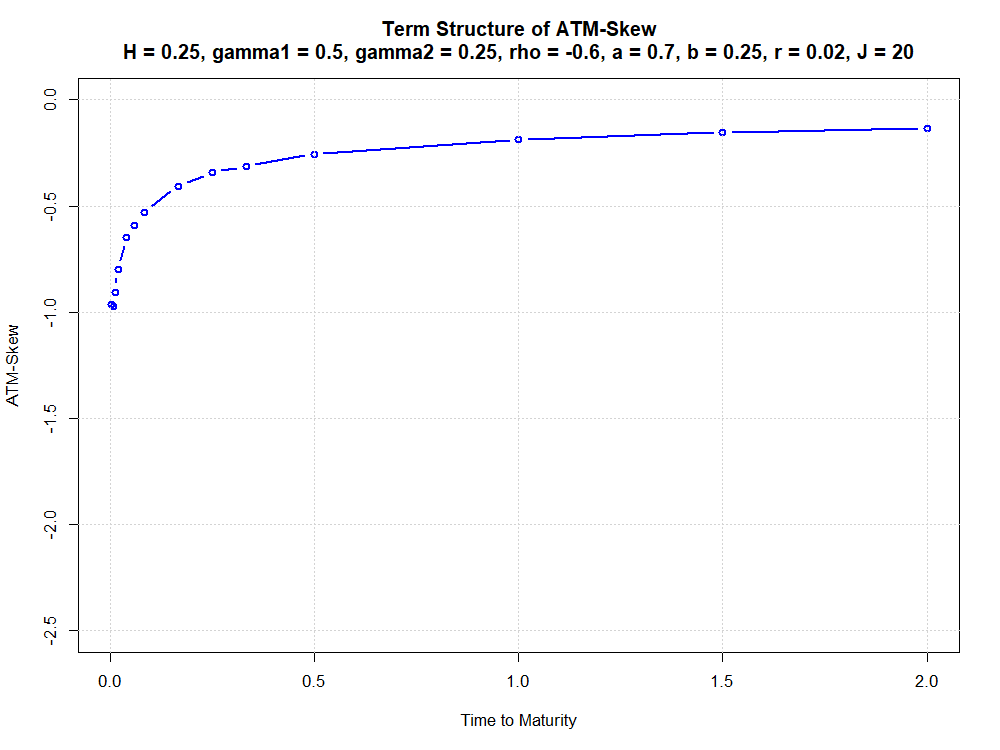
\includegraphics[width=0.45\textwidth]{figures/5.2 Individual Parameter Effects/rho=-0.6_atm_skew.png}
	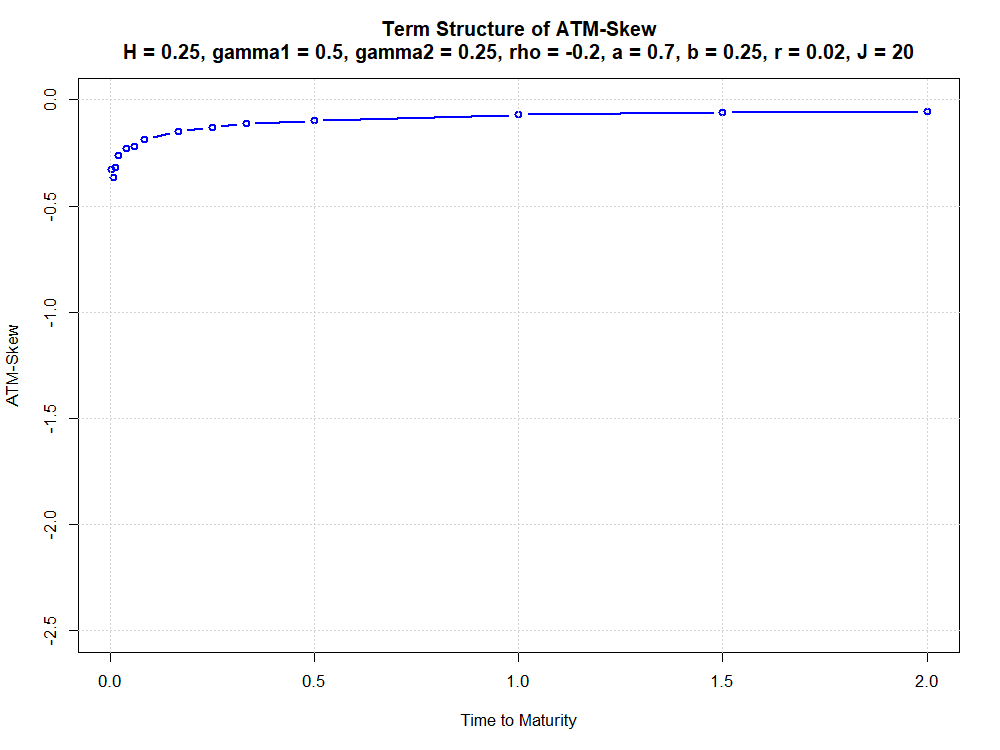
\includegraphics[width=0.45\textwidth]{figures/5.2 Individual Parameter Effects/rho=-0.2_atm_skew.png}
    \caption{Effect of Correlation $\rho$ on the implied volatility surface. Left: $\rho=-0.6$. Right: $\rho=-0.2$.}
    \label{fig:rho_effect}
\end{figure}

\subsubsection*{Effect of Volatility Scale Parameter $a$}
Increasing the volatility scale parameter $a$ amplifies the influence of the latent signal process on the volatility level. This leads to higher implied volatilities in the wings, i.e., for deep in- or out-of-the-money options. The ATM skew magnitude also increases, particularly for short maturities.
\begin{figure}[H]
    \centering
    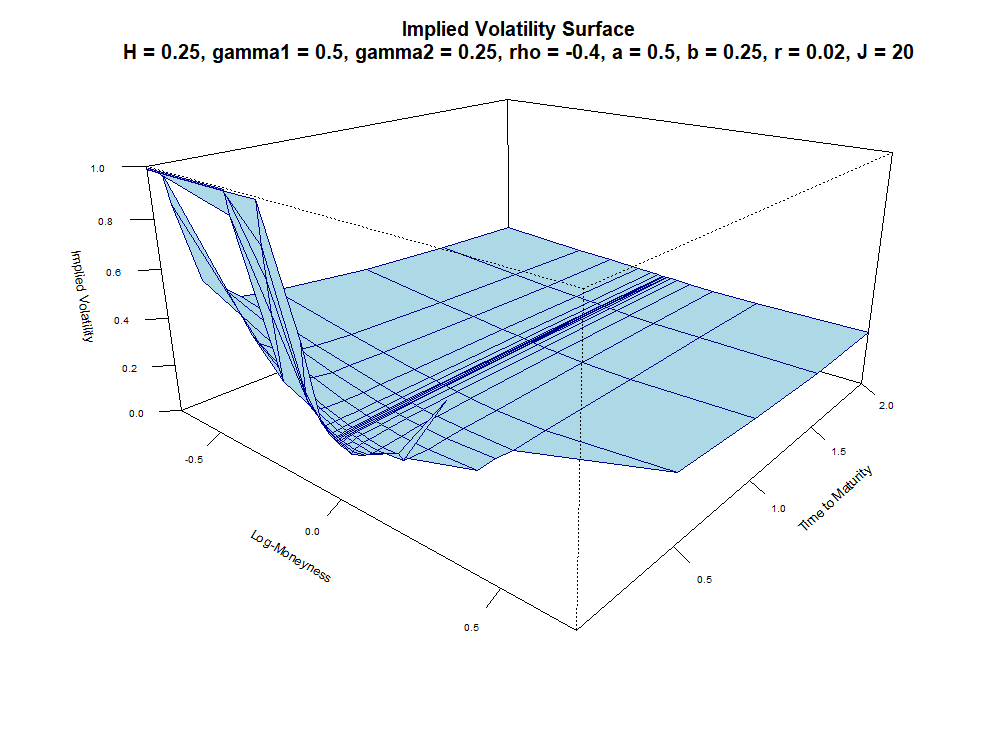
\includegraphics[width=0.45\textwidth]{figures/5.2 Individual Parameter Effects/a=0.5_iv_surface.png}
	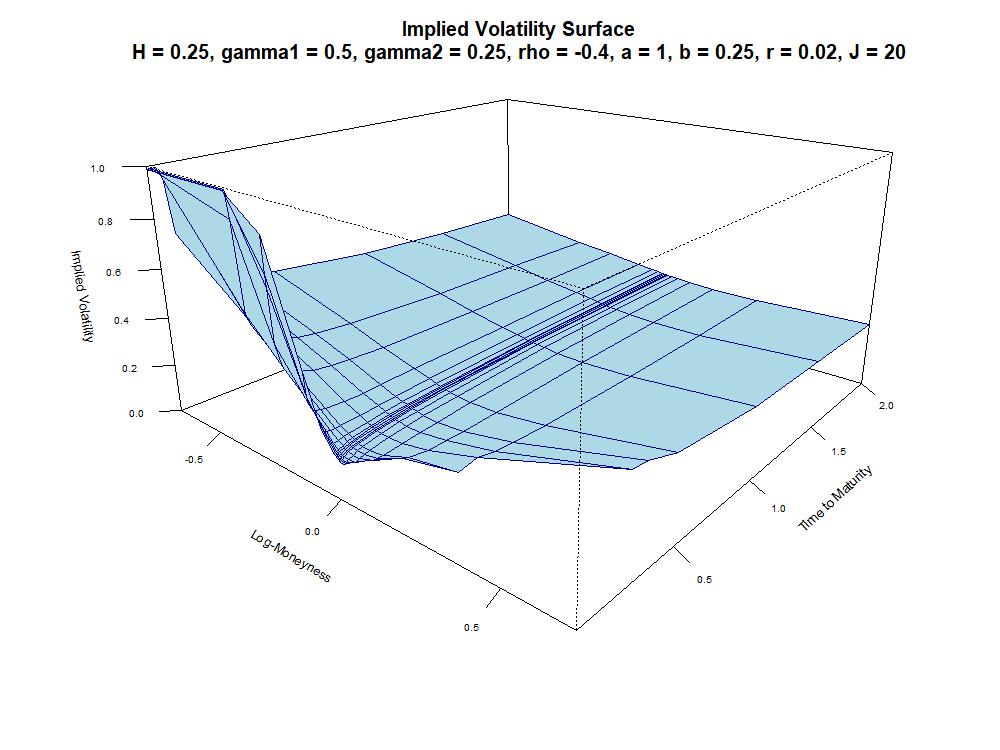
\includegraphics[width=0.45\textwidth]{figures/5.2 Individual Parameter Effects/a=1.0_iv_surface.png}
	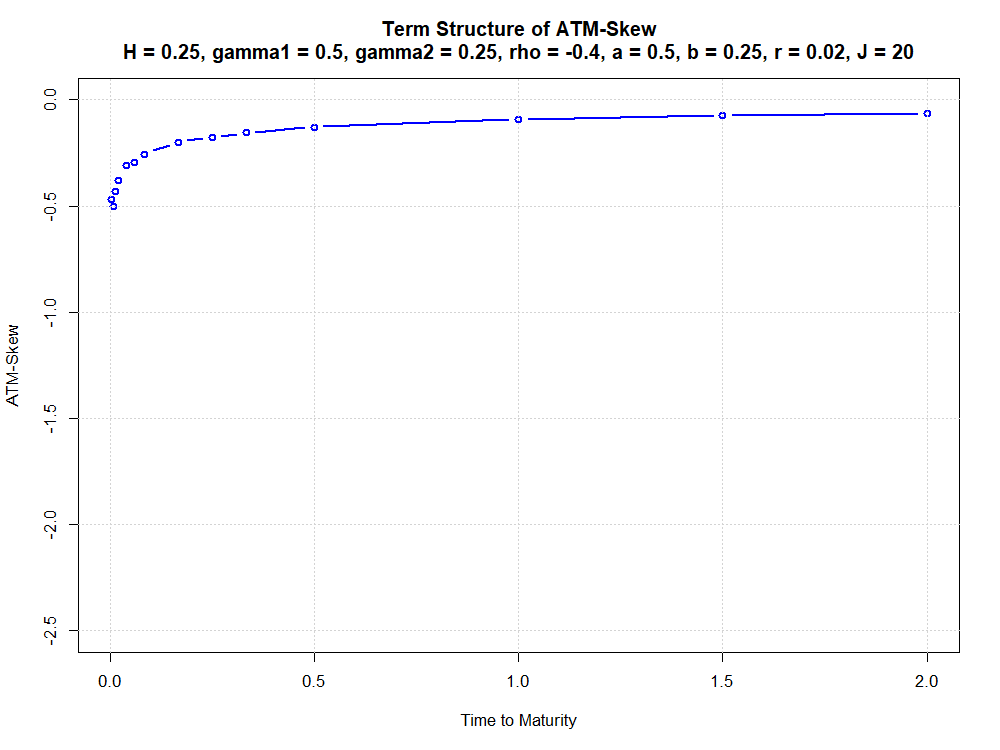
\includegraphics[width=0.45\textwidth]{figures/5.2 Individual Parameter Effects/a=0.5_atm_skew.png}
	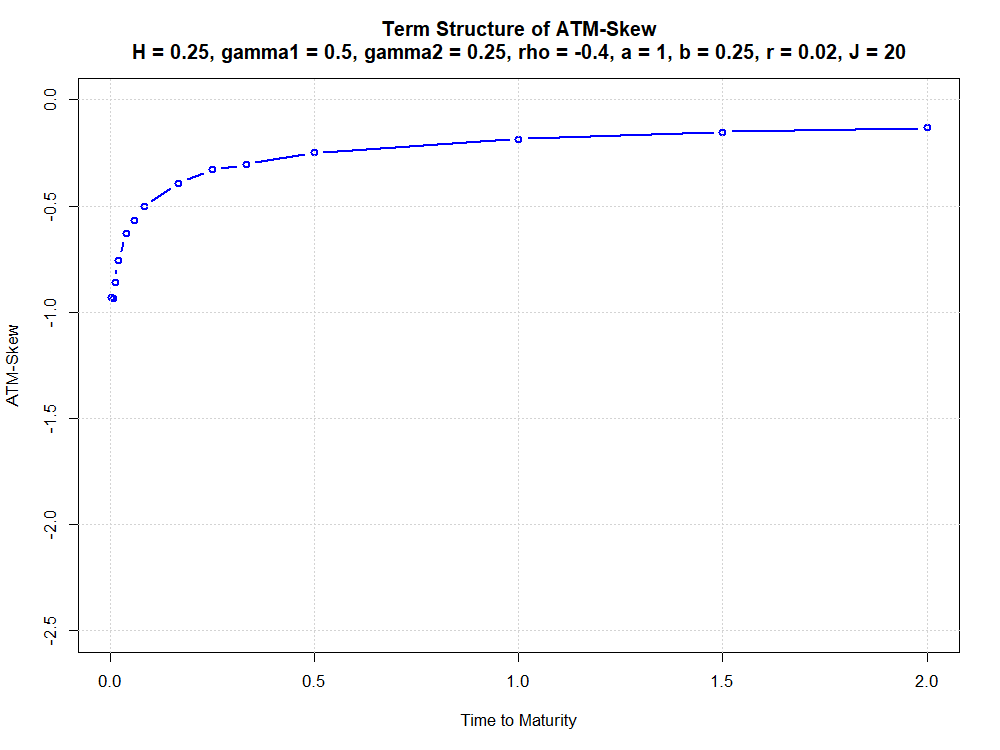
\includegraphics[width=0.45\textwidth]{figures/5.2 Individual Parameter Effects/a=1.0_atm_skew.png}
    \caption{Effect of Volatility Scale Parameter $a$ on the implied volatility surface. Left: $a=0.5$. Right: $a=1.0$.}
    \label{fig:a_effect}
\end{figure}

\subsubsection*{Effect of Base Volatility Level $b$}
Raising the base volatility level $b$ shifts the entire implied volatility surface upward. Additionally, it increases the magnitude of the slope in the log-log regression of the ATM skew, suggesting a steeper power-law decay. This reflects a stronger term structure effect in the skew.
\begin{figure}[H]
    \centering
    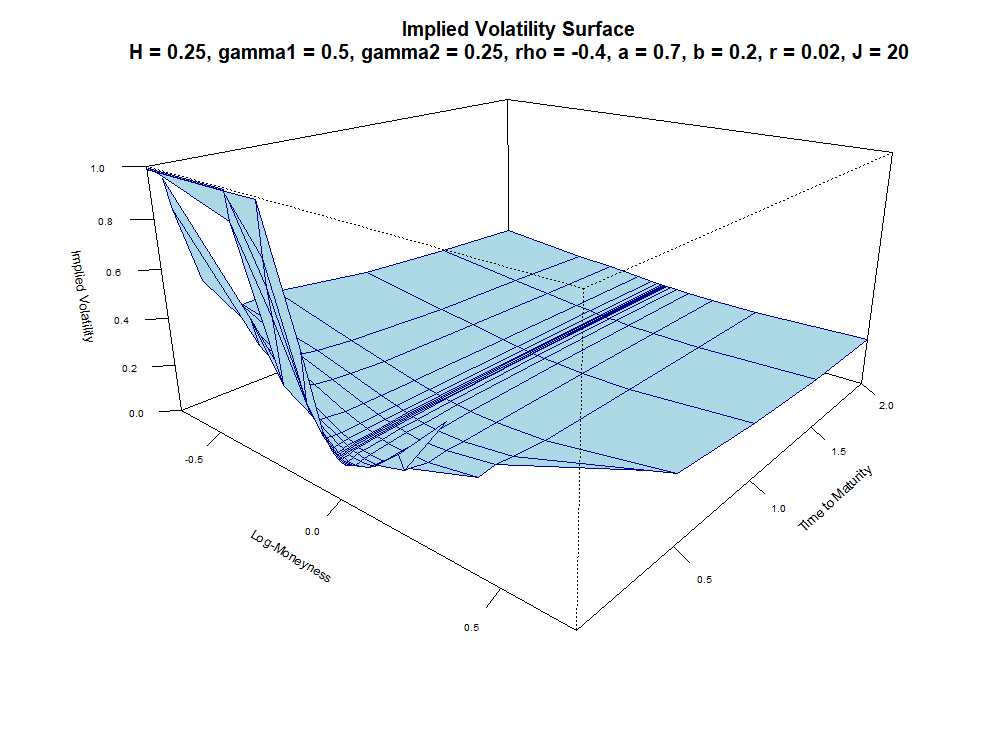
\includegraphics[width=0.45\textwidth]{figures/5.2 Individual Parameter Effects/b=0.2_iv_surface.png}
	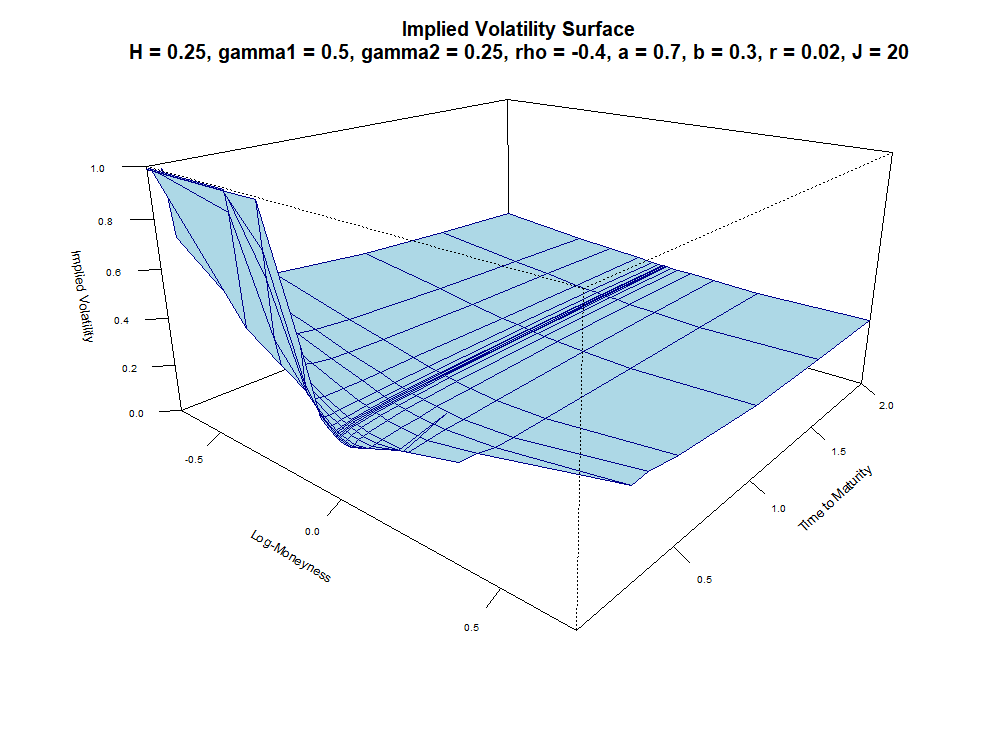
\includegraphics[width=0.45\textwidth]{figures/5.2 Individual Parameter Effects/b=0.3_iv_surface.png}
	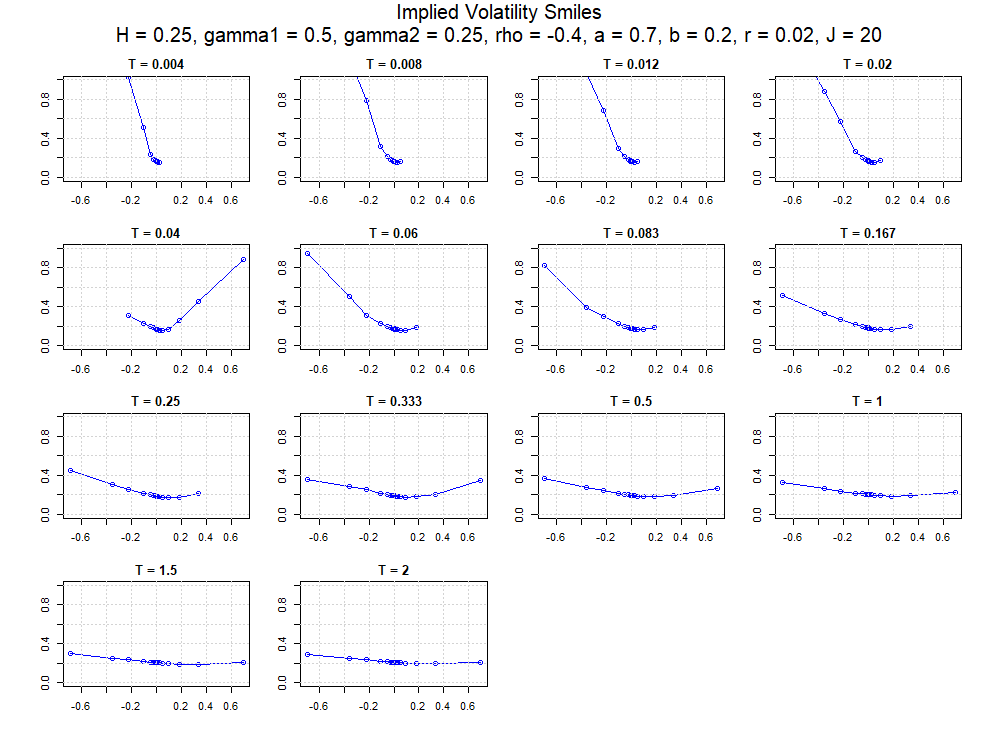
\includegraphics[width=0.45\textwidth]{figures/5.2 Individual Parameter Effects/b=0.2_iv_smiles.png}
	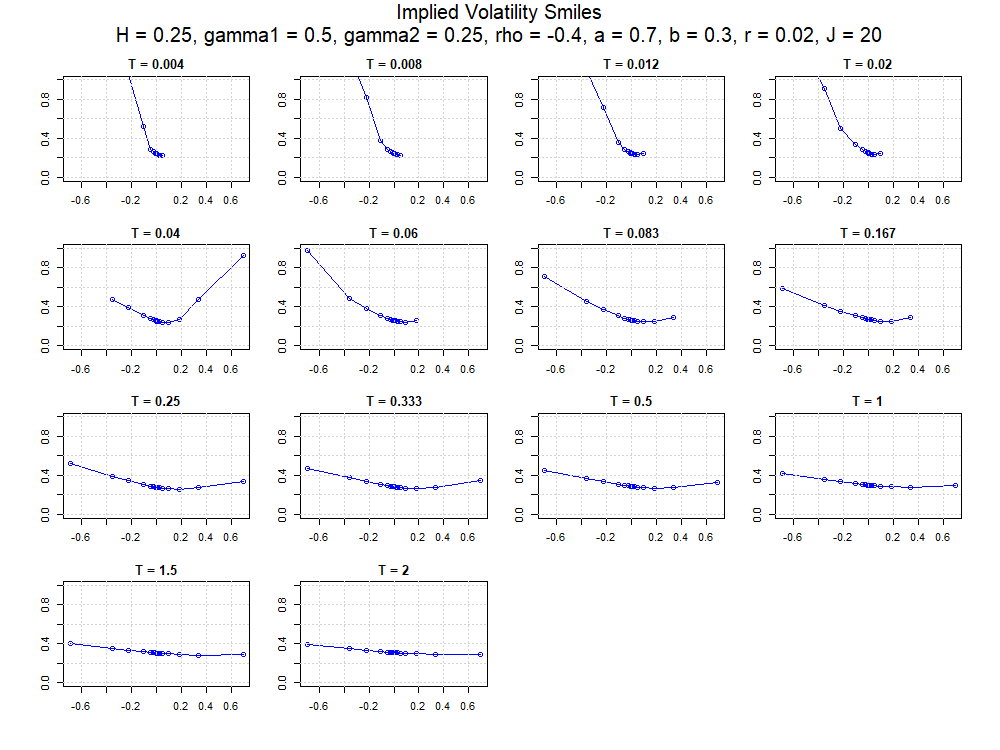
\includegraphics[width=0.45\textwidth]{figures/5.2 Individual Parameter Effects/b=0.3_iv_smiles.png}
    \caption{Effect of Base Volatility Level $b$ on the implied volatility surface. Left: $b=0.2$. Right: $b=0.3$.}
    \label{fig:b_effect}
\end{figure}

\subsubsection*{Effect of Persistence Parameter $\gamma_2$}
Higher values of $\gamma_2$ increase the persistence in the signal process. This reduces the short-term ATM skew and flattens the power-law slope in the log-log skew regression. Overall, increased persistence slightly lowers the implied volatility surface, especially at short maturities.

\subsubsection*{Effect of Risk-Free Interest Rate $r$}
Changes in the risk-free interest rate $r$ have no effect on the implied volatility surface, as expected under risk-neutral pricing. This serves as a consistency check for the numerical implementation.


\subsection{Success Rate Analysis} \label{subsec:SuccessRateAnalysis}

To evaluate model performance, this section analyzes the proportion of simulation scenarios that satisfy the five quality criteria defined in Section~\ref{subsec:SimulationQualityCriteria}. Each scenario corresponds to a unique configuration of model parameters. A scenario is considered successful if all five criteria are met.

\subsubsection*{Parameter Grid Used in the Simulation Study}
The simulation study was based on a structured grid of parameters chosen to reflect realistic variation in volatility dynamics. In total, 18{,}225 scenarios were evaluated, where the following values were tested:
\begin{itemize}
    \item Roughness index $H \in \{0.05, 0.10, 0.15, 0.20, 0.25, 0.30, 0.35, 0.40, 0.45\}$
    \item Persistence parameter $\gamma_2 \in \{0.05, 0.10, 0.15, 0.20, 0.25, 0.30, 0.35, 0.40, 0.45\}$
    \item Volatility scale parameter $a \in \{0.5, 0.7, 1.0, 1.4, 2.0\}$
    \item Base volatility level $b \in \{0.10, 0.15, 0.20, 0.25, 0.30\}$
    \item Correlation $\rho \in \{-0.8, -0.7, -0.6, -0.5, -0.4, -0.3, -0.2, -0.1, 0\}$
\end{itemize}
The parameter $\gamma_1$ was computed using the identity
\begin{equation*}
    \gamma_1 = H + \tfrac{1}{2} - \gamma_2,
\end{equation*}
according to Equation~\eqref{eq:HurstIndex} to ensure the correct asymptotic behavior of the hypergeometric kernel.

\subsubsection*{Overall Success Rates}
Put-call parity is satisfied in 93\% of all simulations, while the smile convexity criterion is met in 66\% of cases. The skew negativity and skew monotonicity criteria are fulfilled in 99\% and 96\% of all scenarios, respectively. The power-law fit criterion is satisfied in 70\% of cases, and 54\% of all scenarios meet all five criteria simultaneously. Table~\ref{tab:OverallSuccessRates} summarizes the proportion of scenarios satisfying each individual criterion.
\begin{table}[H]
    \centering
    \small
    \begin{tabular}{lccccc}
        \toprule
        Criterion & Put-Call Parity & Smile Convexity & Skew Negative & Skew Increasing & Skew Power Law \\
        \midrule
        Success Rate & 93\% & 66\% & 99\% & 96\% & 70\% \\
        \bottomrule
    \end{tabular}
    \caption{Overall success rates across all simulation scenarios.}
    \label{tab:OverallSuccessRates}
\end{table}

Put-Call Parity success rate drops significantly for higher levels of $a$, other than that, it improves for higher levels of $H$, higher levels of $\gamma_2$, lower levels of $\rho$, and lower levels of $b$.

Smile Convexity significantly worsens for strongly negative $\rho$ and higher levels of $a$. Additionaly, it is marginally optimal at $H \in [0.1, 0.15]$ and larger $b$, while $gamma_2$ has no effect on smile convexity.

Skew negativity has very high acceptance rates close to 100\% across all parameter choices, except for $\rho = 0$.

Skew increase improves for lower levels of $H$. Otherwise, acceptance rates are very high for all parameter choices, given correlation is negative.

Skew power law fit improves lower levels of $H$, lower $\rho$, and higher $b$. The acceptance rate significantly drops for $a = 2$, while it reaches its optimum at $a = 1$.


\subsubsection*{Effect of the Roughness Parameter \texorpdfstring{$H$}{H}}
The roughness index $H$ has a noticeable impact. The put-call parity success rate increases monotonically from 84\% at $H = 0.05$ to 99\% at $H = 0.45$. However, smile convexity shows a non-monotonic pattern, peaking at $H = 0.10-0.25$ (69-71\%) and dropping to 58\% at $H = 0.45$. The skew negativity criterion is satisfied to almost at least 99\% across all $H$, with 100\% success rate at $H = 0.15-0.20$. The skew increase criterion has a higher success rate with lower roughness parameter, ranging from 90\% at $H = 0.45$ to 100\% at $H = 0.05-0.15$. The power-law fit is also satisfied at a higher rate for lower values of $H$, with highest rate of success at $H = 0.05$ (77\%), and lowest at $H = 0.45$ (57\%). Overall, $H \in [0.10, 0.25]$ appears to offer the best trade-off across criteria.

\subsubsection*{Effect of the Persistence Parameter \texorpdfstring{$\gamma_2$}{gamma2}}
The parameter $\gamma_2$ controls the long memory property of the mixing kernel. Success rates remain remarkably stable across all values $\gamma_2 = 0.05,\ldots,0.45$. For $\gamma_2$, put-call parity rises from 90\% to 96\%, while smile convexity declines slightly from 67\% to 64\%. The skew negativity has a constant success rate (99\%) across all values of $\gamma_2$, while the skew increasing marginally falls for increasing values of $\gamma_2$. The power-law fit is almost constant across the full range (70\%-71\%). Overall, the persistence parameter has very little effect on the overall success rate, with slightly better results for lower values $\gamma_2 \in [0.05, \ldots, 0.25]$.

\subsubsection*{Effect of the Volatility Amplification Parameter \texorpdfstring{$a$}{a}}
The volatility scale parameter $a$ has strong influence on simulation quality. For $a \leq 1.4$, the model performs well, with most criteria satisfied in over 80\% of scenarios. However, at $a = 2.0$, simulation performance degrades significantly: smile convexity drops to 2\%, put-call parity to 70\%, and power-law fit to 13\%. This suggests that excessive amplification of volatility leads to unstable surfaces, and that $a$ should be kept below 1.4. Overall, best results are obtained using $a \in [0.5, 1]$.

\subsubsection*{Effect of the Base Volatility Level \texorpdfstring{$b$}{b}}
The parameter $b$ affects the level of volatility in the model. Higher $b$ values improve smile convexity (from 52\% at $b = 0.10$ to 72\% at $b = 0.30$) and support skew criteria, but slightly reduce put-call parity satisfaction (from 98\% to 88\%). Overall, $b \in [0.20, 0.30]$ offers the best balance.

\subsubsection*{Effect of the Correlation Parameter \texorpdfstring{$\rho$}{rho}}
The correlation $\rho$ between the Brownian motions driving the asset and the signal process has a strong effect. Put-call parity improves with a stronger leverage effect (up to 100\% at $\rho = -0.8$), while the smile convexity improves monotonically for less correlated Brownian motions. Skew negativity and skew increasing are met at a 100\% rate for negative correlations, but not for zero correlation. The power-law fit has higher success rate improves for stronger negative correlation. Overall, negative values of $\rho > -0.7$ have acceptable success rates with the best results at $\rho \in [-0.6, -0.2]$.


\subsection{Optimal Parameter Ranges}

Based on the success rate analysis, the following parameter regions yield the best simulation performance:
\begin{itemize}
    \item \textbf{Roughness index $H$:} Best performance occurs for $H \in [0.10, 0.25]$.
    \item \textbf{Volatility amplification $a$:} Stability breaks down for $a > 1.4$; optimal range is $a \in [0.5, 1]$.
    \item \textbf{Base volatility level $b$:} Best results for $b \in [0.20, 0.30]$.
    \item \textbf{Correlation $\rho$:} Optimal range: $[-0.6, -0.2]$.
    \item \textbf{Kernel parameters $\gamma_1$, $\gamma_2$:} No strong sensitivity observed; model is robust within the tested range.
\end{itemize}
These parameter ranges provide the foundation for model calibration and surface fitting in Section~\ref{sec:Calibration}.

\begin{figure}[H]
    \centering
    \includegraphics[width=0.45\textwidth]{figures/5.4 Optimal Parameter Ranges/optimal_example_iv_surface.png}
    \includegraphics[width=0.45\textwidth]{figures/5.4 Optimal Parameter Ranges/optimal_example_iv_smiles.png}
    \includegraphics[width=0.45\textwidth]{figures/5.4 Optimal Parameter Ranges/optimal_example_atm_skew.png}
    \includegraphics[width=0.45\textwidth]{figures/5.4 Optimal Parameter Ranges/optimal_example_atm_skew_log.png}
    \caption{Implied volatility surface, smiles and ATM skew.}
    \label{fig:OptimalExampleSurface}
\end{figure}

The surface shown in Figure~\ref{fig:OptimalExampleSurface} was generated using:
\[
H = 0.20, \quad a = 0.7, \quad b = 0.25, \quad \rho = -0.4, \quad \gamma_2 = 0.25, \quad \gamma_1 = H + 0.5 - \gamma_2.
\]
This configuration satisfies all five quality criteria and produces a realistic surface shape consistent with observed market data.